\documentclass[
    11pt,
    a4paper,
    egregdoesnotlikesansseriftitles,
    toc=chapterentrywithdots,
    twoside,openright,
    titlepage,
    parskip=half,
    headings=normal,  % reduces heading size
    listof=totoc,
    bibliography=totoc,
    index=totoc,
    captions=tableheading,  % caption below table
    chapterprefix,
    listof=flat,
    final
]{scrbook}

\makeindex
% details about your thesis
\newcommand{\titel}{My very fancy thesis title.}
\newcommand{\artderarbeit}{Bachelorarbeit}  % {Bachelorarbeit,Masterarbeit}
\newcommand{\autor}{Lukas Welsch}
\newcommand{\studiengang}{Informatik}  % {Informatik,Wirtschaftsinformatik,Medieninformatik}
\newcommand{\matrikelnr}{3201095}
\newcommand{\erstgutachter}{Prof.\,Dr.~Korbinian Riedhammer}
\newcommand{\zweitgutachter}{Prof.\,Dr.~Jens Albrecht}
\newcommand{\betreuer}{Dipl. Ing.\,~Andreas Sachs}
\newcommand{\unternehmen}{Sopra Financial Technology GmbH}
\newcommand{\logo}{figures/TH-Nuernberg-RGB.png}
\newcommand{\keywords}{hot, fuzz}
 

% custom head and foot
\usepackage[automark]{scrlayer-scrpage}
\pagestyle{scrheadings}
\ihead{\headmark}
\chead{}
\ohead{\pagemark}
\renewcommand*\chaptermarkformat{\chapappifchapterprefix{\ }% 
  \thechapter.\enskip}

\RedeclareSectionCommand[tocindent=0pt]{section}
\RedeclareSectionCommand[tocindent=0pt]{subsection}
%\RedeclareSectionCommand[tocnumwidth=70pt]{chapter}

\usepackage{scrhack}

% other packages
\usepackage[utf8]{inputenc}
\usepackage[T1]{fontenc}
\usepackage{lmodern,relsize,textcomp,csquotes}
\usepackage{amsmath,amsfonts}
\usepackage[english,ngerman]{babel}  % flip for German thesis
\usepackage[final]{graphicx}
\usepackage{setspace,geometry,xcolor}
\usepackage{makeidx}
\usepackage{paralist,ifthen,todonotes}
\usepackage{url}
\usepackage[toc]{glossaries}
\usepackage{pdfpages}

% table setup
\usepackage{longtable}
\usepackage{array}
\usepackage{ragged2e}
\usepackage{lscape}

% pdf hyperref
\usepackage[
    bookmarks=true,
    bookmarksopen=true,
    bookmarksnumbered=true,
    bookmarksopenlevel=1,
    pdftitle={\titel},
    pdfauthor={\autor},
    pdfcreator={\autor},
    pdfsubject={\titel},
    pdfkeywords={\keywords},
    pdfpagelabels=true,
    colorlinks=true,
    linkcolor=red,
    urlcolor=magenta,
    anchorcolor=black,
    citecolor=cyan,
    filecolor=magenta,
    menucolor=red,
    plainpages=false,
    hypertexnames=true,
    linktocpage=true,
]{hyperref}


% configure your listings style
\usepackage{listings}
\lstset{
	tabsize=3,
	extendedchars=true,
	frame=single,
	showstringspaces=true,
	numbers=left,
	numberstyle=\small,
	breakautoindent=true
}

% page setup
% \setlength{\topskip}{\ht\strutbox}
\geometry{paper=a4paper,left=2.5cm,top=3.0cm,bindingoffset=.8cm}
\onehalfspacing
\frenchspacing
\clubpenalty = 10000
\widowpenalty = 10000 
\displaywidowpenalty = 10000

% some commands
\newcommand{\ua}{\mbox{u.\,a.\ }}
\newcommand{\zB}{\mbox{z.\,B.\ }}
\newcommand{\dahe}{\mbox{d.\,h.,\ }}
\newcommand{\bzw}{\mbox{bzw.\ }}
\newcommand{\bzgl}{\mbox{bzgl.\ }}
\newcommand{\eg}{\mbox{e.\,g.\ }}
\newcommand{\ie}{\mbox{i.\,e.\ }}
\newcommand{\wrt}{\mbox{w.\,r.\,t.\ }}
\newcommand{\etal}{\mbox{\emph{et.\,al.\ }}}


% TODO remove if not needed...
\usepackage{blindtext}

% load glossary entries
\makenoidxglossaries
\loadglsentries{glossary}

\begin{document}

\setcounter{secnumdepth}{3}  % numerate subsections
\setcounter{tocdepth}{2}  % ...but don't include them in toc

\frontmatter
\thispagestyle{empty}
\pdfbookmark[1]{Cover}{cov}
\begin{titlepage}

\begin{center}

%\includegraphics[width=\linewidth]{figures/TH-Nuernberg-RGB.png}\\[1cm]
\LARGE{Fakultät Informatik}\\[2cm]

\huge
\textbf{\titel}\\[1cm]
%
\Large
\artderarbeit~im Studiengang \studiengang\\[1cm]
%
\large
vorgelegt von

\Large
\autor\\[0.5cm]
\small
Matrikelnummer \matrikelnr\\[2cm]

\vspace*{\fill}

\large
\begin{tabular}{p{3cm}p{8cm}}\\
Erstgutachter:  & \quad \erstgutachter\\[1.2ex]
Zweitgutachter: & \quad \zweitgutachter\\[1.2ex]
%discomment "Betreuer" and "Unternehmen" for a thesis in a company
Betreuer: & \quad \betreuer\\
Unternehmen: & \quad \unternehmen
\end{tabular}
\end{center}

\begin{center}
\copyright\,\the\year
\end{center}

\vspace{-0.5cm}
\singlespacing
\small
\noindent Dieses Werk einschließlich seiner Teile ist \textbf{urheberrechtlich geschützt}.
Jede Verwertung außerhalb der engen Grenzen des Urheberrechtgesetzes ist ohne Zustimmung des Autors unzulässig und strafbar.
Das gilt insbesondere für Vervielfältigungen, Übersetzungen, Mikroverfilmungen sowie die Einspeicherung und Verarbeitung in elektronischen Systemen.

\end{titlepage}
\cleardoublepage

% download the following form and complete it (hit save in your editor)
% https://intern.ohmportal.de/fileadmin/Gelenkte_Doks/Abt/SZS/SB/SB_0050_FO_Pruefungsrechtliche_Erklaerung_und_Erklaerung_zur_Veroeffentlichung_der_Abschlussarbeit_public.pdf
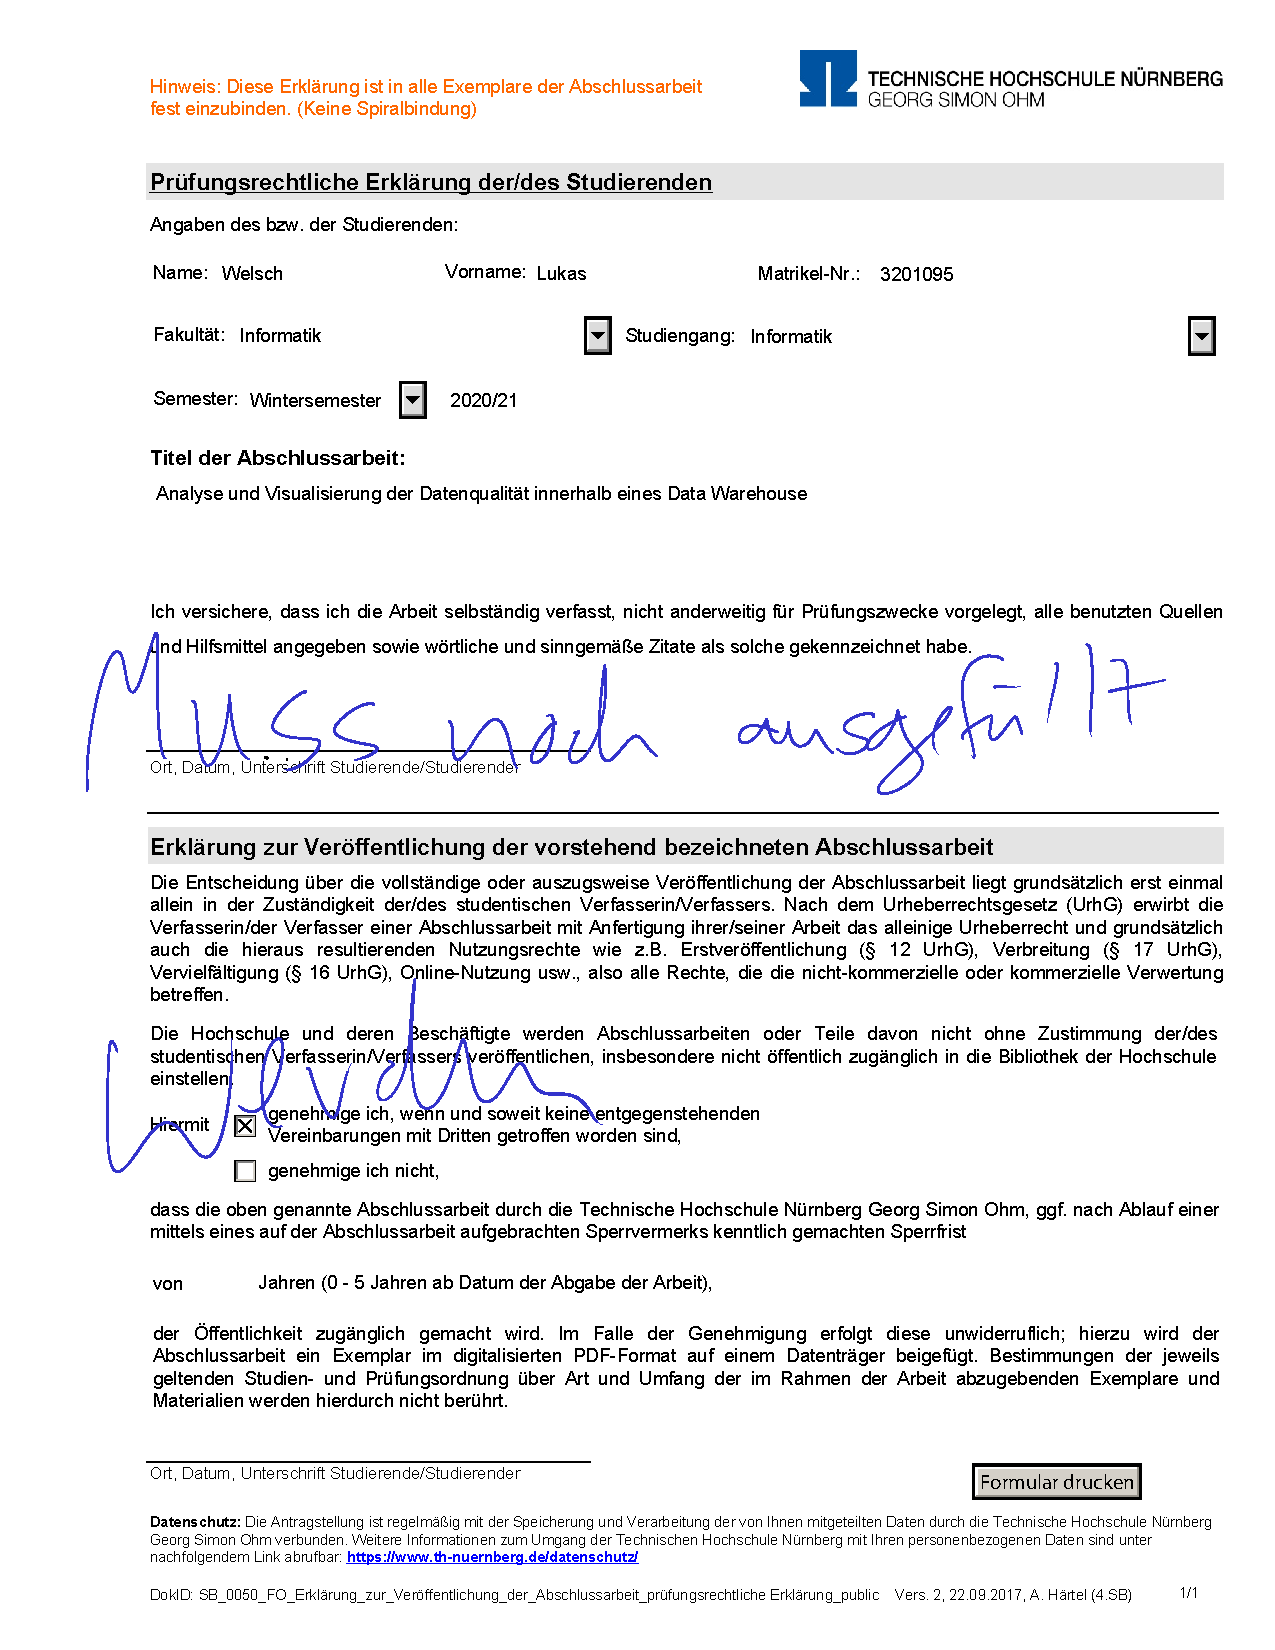
\includepdf{SB_0050_FO_Pruefungsrechtliche_Erklaerung_und_Erklaerung_zur_Veroeffentlichung_der_Abschlussarbeit_public.pdf}\cleardoublepage

\thispagestyle{empty}
\section*{Kurzdarstellung}
\label{sec:kurzdarstellung}
Kurze Zusammenfassung der Arbeit, höchstens halbe Seite.
Deutsche Fassung auch nötig, wenn die Arbeit auf Englisch angefertigt wird.

\blindtext


\section*{Abstract}
\label{sec:abstract}
\emph{Only if thesis is written in English.}

\blindtext
\cleardoublepage

\tableofcontents

\mainmatter
\chapter{Einleitung}\label{ch:intro}

%You may have read about similar things in \cite{Goodliffe2007}.
%You can also write footnotes.\footnote{Footnotes will be positioned automatically.}
%It is possible to reference glossary entries as \gls{library} as an example.




- Kann mit Hilfe von ML-Verfahren berechnet werden, ob Risikobewertungen über Kunden aktualisiert werden müssen? 
% externe Dienstleister bündeln die Informationen mehrerer Kreditvergeber. 
% Deshalb werden die Daten von dort vermutlich immer akurater sein und können nicht ersetzt werden
- Können die vorliegenden MetaDaten visualisiert werden, sodass Erkenntnisse zur (Prozess)-Qualität gewonnen werden können? 

\cite{d.kelleher2015a}
\cite{d.kelleher2015}

%IDEEN
%versch. Arten visualisieren und dann selbst entscheiden bzw Entscheidungen von Experten mit einfließen lassen
%Anpassung der Adressen aus den letzten Jahren (Durchschnitt wie oft wird Kundenstammdaten aktualisiert)



% Problematisch ist, dass die IT-Systeme so gestaltet sind, dass diese Freitextfelder verfügbar sind, sodass erst keine Rechtschreibfehler entstehen können. 
% Allerdings steht die Bank vor dem Problem die Daten schon erhoben zu haben und benötigt jetzt eine Lösung, um diese auszubessern. 


\chapter{Grundlagen}\label{ch:data}

\section{Definition von Datenqualität}
Datenqualität wird in der Literatur auf verschiedene Arten definiert. 
Viele Datenqualitätsstudien verwenden Korrektheit als einziges Datenqualitätsmerkmal. \cite{wang1996}
Datenqualität umfasst jedoch nicht nur die Korrektheit von Daten, sondern auch anderen Dimensionen. 
Ein Paper von Oliva, Zubcoff und Mazón zeigt den Einfluss von anderen Dimensionen, wie zb. Vollständigkeit auf die Erkennungsrate von Klassifikatoren \cite{espinosaoliva2011} Die Autoren schlagen vor den Aufbereitungsprozess und vor allem Datenqualität nicht nur auf die Korrektheit von Daten zu beziehen sondern auch auf die anderen Datenqualitätsdimensionen zu achten.

\subsection{Datenqualitätsdimensionen}
Die Dimensionen Richtigkeit, Vollständigkeit, Konsistenz und Aktualität werden in den meisten Veröffentlichungen genannt, allerdings gibt es keinen Standard, weder im Bezug auf die verwendeten Dimensionen, noch die Definition der Dimensionen. \cite{scannapieco2002}
Da keine allgemeine Empfehlung zur Verwendung von Dimensionen existiert werden in dieser Arbeit die Datenqualitätsdimensionen verwendet, die in den meisten Veröffentlichungen auftauchen.
Dies kann dem Paper von Scannapieco und Catarci entnommen werden. 
Diese Dimensionen sind für die Auswertung der Methoden im Rahmen der Arbeit geeignet. 
Jede dieser Datenqualitätsdimensionen umfasst eine Facette der Datenqualität und werden im Folgenden nach Wand und Wang beschrieben \cite{wand1996}. \\

\textbf{Richtigkeit} \\
Richtigkeit wird als Gleichheit zwischen zwei Werten definiert, sodass die Daten die Wirklichkeit korrekt repräsentieren. 
Beispiel: Eine Person mit dem Namen Max Mustermann ist als Mx Mustermann abgespeichert. 
Die gespeicherten Daten repräsentieren nicht die Wirklichkeit, sie sind somit nicht richtig. \\

\textbf{Aktualität / temporäre Richtigkeit} \\
Als Spezialisierung der Richtigkeit kann die temporäre Richtigkeit gesehen werden, die richtige Repräsentation zu einem bestimmten Zeitpunkt oder Zeitspanne beschreibt. 
Die temporäre Richtigkeit zum aktuellen Zeitpunkt wird auch als Aktualität bezeichnet. \\

\textbf{Vollständigkeit} \\
Die Daten sind umfangreich genug für die jeweilige Aufgabe. \cite{wang1996} 
Da ein Data Warehouse aus relationalen Datenbanken besteht, wird die Vollständigkeit im Folgenden auf relationale Datenbanken bezogen.
Die Vollständigkeit wird von \cite{pipino2002} in drei Klassen kategorisiert.
\begin{itemize}
 \item Schema: Grad der Daten, die nicht im Schema fehlen
 \item Spalte: Anzahl der fehlenden Werte innerhalb einer Spalte
 \item Population: Wenn eine Spalte alle 16 Bundesländer beinhalten sollte, aber nur 14 vorhanden sind, dann herrscht Populationsunvollständigkeit \\
\end{itemize} 

\textbf{Konsistenz} \\
Die gleichen (redundanten) Datensätze haben die gleichen Werte in verschiedenen Tabellen. 
Ein Beispiel für Konsistenz ist die referentielle Integrität, die sicherstellt, dass Datensätze nur auf existierende Datensätze verweisen. 
\\ % \textbf{Appropriate Amount of Data, Believability, }

Für diese Arbeit stehen die Dimensionen Richtigkeit, Aktualität und Vollständigkeit im Vordergrund. 
Dies liegt daran, dass eine Konsistenzprüfung von einem Datenbanksystem automatisch vorgenommen wird. 
Es ist deshalb bei relationalen Daten in der dritten Normalform nicht notwendig diese auf die Konsistenz zu prüfen, da durch die Verwendung der Normalform Redundanzen ausgeschlossen werden. % TODO Quelle Finden!
In einem Data Warehouse werden Daten hingegen in sogenannten Data Marts redundant gespeichert, um eine höhere Leseperformance für die einzelnen Endanwendungen bieten zu können. %TODO Kapitel Alternative DW/BI Architectures
Allerdings können Probleme, die durch Data Marts entstehen einfach mit einer richtigen Modellierung behoben werden. \cite{kimball2002}

In dem vorliegendem Data Warehouse existiert eine Data Vault Architektur. 
In dieser werden die Daten aus Performancegründen redundant abgespeichert. 
Deshalb kann es zu Inkonsistenzen im Datensatz führen. \cite{bolt2020}
Hierfür existiert bereits eine Methode in der Data Warehouse Abteilung.
Dabei werden die Daten zusammengeführt und überprüft, ob Datensätze mit dem gleichen Schlüssel unterschiedliche Werte besitzen. 
Obwohl dieses Szenario in der Realität selten eintritt, ist eine solche Prüfung für die Inkonsistenzvermeidung signifikant. 

\subsection{Metriken der Dimensionen}
Um diese eher abstrakten Definitionen messbar zu machen haben sich einige Verfahren etabliert.
Diese lassen sich grob in die Kategorien subjektiv und objektiv aufteilen, vgl. \autoref{fig:subjektiv} nach Pipino. 


Bei den subjektiven Verfahren wird die vorherrschende Datenqualität durch Experten geschätzt. 
%Dieses Verfahren ist allerdings nicht nur zeitaufwendig für die Experten, sondern ist auch fehleranfällig. \textcolor{red}{\textbf{HIERZITATANGEBEN}} \cite{}
Eine weitere Möglichkeit besteht darin objektive Verfahren zu verwenden, bei denen mit Hilfe von mathematischen Funktionen die Datenqualität berechnet oder geschätzt wird. 

Des weiteren gibt es ein kombiniertes Verfahren, bei dem Grenzwerte von Experten geschätzt und anschließend durch mathematische Funktionen abgeglichen werden. 
Das kombinierte Verfahren kann durch Quadrate visualisiert werden, die an der y-Achse die subjektive Bewertung und auf der x-Achse die objektive Bewertung zeigen, vgl. \autoref{fig:subjektiv}. 
Diese sind aufgeteilt in hohe bzw. niedrige Datenqualität.
Ziel einer Datenqualitätsmaßnahme ist es sowohl eine hohe subjektive als auch hohe objektive Datenqualität zu erlangen.
Bei einer guten Datenqualität liegt das Ergebnis im IV. Quadrant. \cite{pipino2002} 


\begin{figure}[hbt!]
\centering
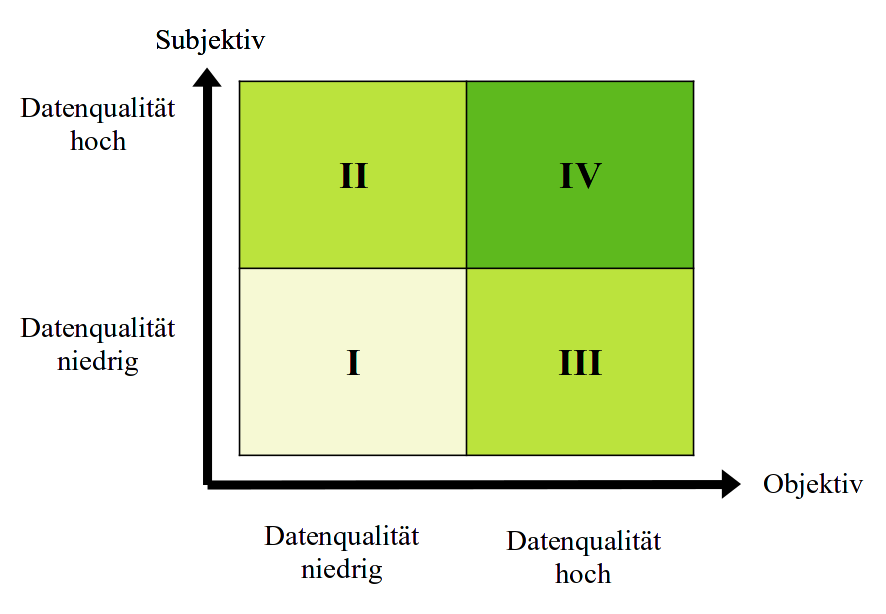
\includegraphics[width=100mm,scale=1]{content/subjektiv_objektiv.png}
\caption{Eigene Darstellung der Auswertung von objektiven und subjektiven Verfahren, basiert auf der Abbildung von \cite{pipino2002}}\label{fig:subjektiv}
\end{figure}




\section{Standardisierter Prozess}
Der Erfolg von Projekten kann durch die Verwendung eines standardisierten Prozesses deutlich gesteigert werden.
Einer der für Data Mining Projekte am weitesten verbreitet und eingesetzte Prozess ist der Cross Industry Standard Process for Data Mining (CRISP-DM). \cite{d.kelleher2015crispdm}
Der Prozess beinhaltet die Phasen, die nötig sind, um ein Data Mining Projekt durchzuführen. 
Des weiteren ist definiert, welche Aufgaben in der jeweiligen Phase anfallen und welche Ergebnisse die Phasen hervorbringen \cite{wirth2000}.

\begin{figure}[h]
\centering
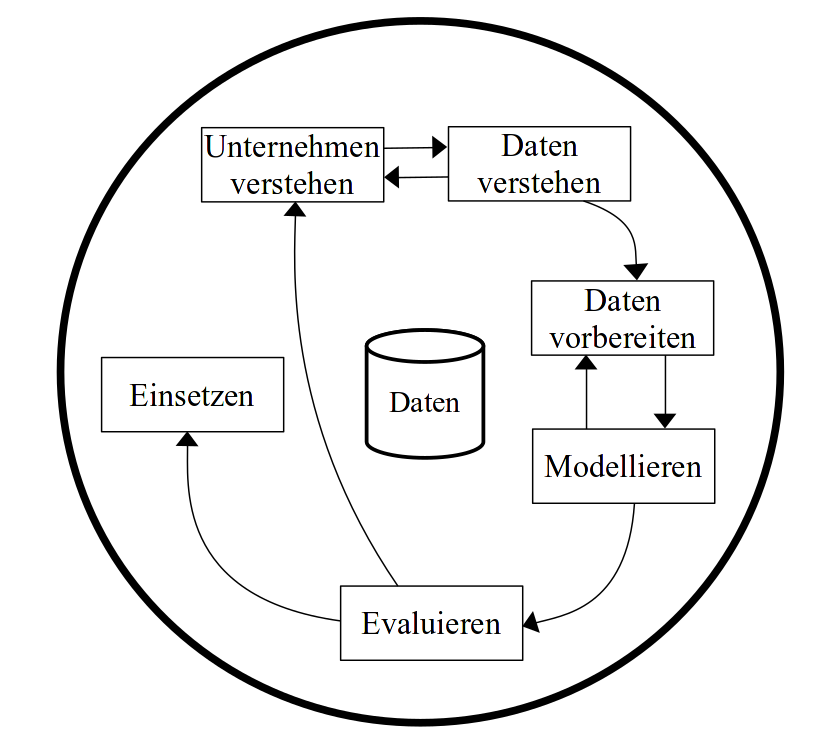
\includegraphics[width=100mm,scale=1]{content/CRISP-Prozess.png}
\caption{Eigene Darstellung des CRISP-DM, basiert auf der Abbildung von \cite{wirth2000}}\label{fig:crisp}
\end{figure}
In der \autoref{fig:crisp} sind die Phasen und ihre Ablaufreihenfolge zu sehen. 
In der Grafik ist zu erkennen, dass es sich bei dem CRISP-DM um einen iterativen Prozess handelt.
Auch in dieser Bachelorarbeit wird nach diesem Vorgehensmodell gearbeitet. 
Die Bestandteile des Modells finden sich in den einzelnen Kapiteln wieder. 
Für die Visualisierung und das Erstellen des Dashboards wird die Phase Modellieren durch Visualisieren ersetzt. 
\\

Die Bestandteile des Prozesses sind: \\
\begin{enumerate}
 \item \textbf{Unternehmen verstehen} \\
 Bei diesem Punkt ist die Aufgabe herauszufinden, welches Problem das Unternehmen versucht zu lösen \cite{d.kelleher2015crispdm}.
 
 Das Verständnis für das Problem des Unternehmens wird in dieser Bachelorarbeit in \autoref{ch:anforderungen} mit Hilfe einer Stakeholder-Analyse erlangt. Hierbei werden die betroffenen Personen untersucht und deren Wünsche aufgezeigt. Als Ergebnis werden drei mögliche Verfahren skizziert, die anschließend genauer erläutert werden.  
 
 \item \textbf{Daten verstehen} \\
 Um die Probleme mit Hilfe von Daten lösen zu können, müssen die vorhandenen Daten genau verstanden werden. Es ist wichtig zu verstehen, welche Daten in welcher Quelle vorhanden sind und um welche Datenarten es sich handelt. \cite{d.kelleher2015crispdm} 
 
 Diese Phase ist in \autoref{ch:data} umgesetzt. Dort werden die einzelnen Quellen untersucht und die Ausprägungen der Datenattribute analysiert. Des weiteren werden in dieser Phase die für die Lösung des skizzierten Problems die relevanten Daten aus den Quelltabellen ausgewählt. 
 
 \item \textbf{Daten vorbereiten} \\
 In dieser Phase wird die finale Tabelle aus den Quellen konstruiert, die zum Training der ML-Modelle verwendet wird. Typische Aufgaben in dieser Phase sind die Attributauswahl, Datenbereinigung und das Erzeugen von neuen Eigenschaften anhand der bestehenden Daten. \cite{wirth2000} Diese Tabelle wird auch als Analytical Base Table (ABT) bezeichnet \cite{d.kelleher2015crispdm}.
 
 Die Datenvorbereitung geschieht an zwei Stellen in dieser Bachelorarbeit. 
 Die Konstruktion der ABT geschieht in dem \autoref{ch:data} und die Datenbereinigung wird im \autoref{ch:experiments} durchgeführt. %TODO Lieber auch in dem Kapitel Daten mitmachen? 
 
 \item \textbf{Modellieren} \\
 In dieser Phase werden verschiedene ML-Modelle ausgewählt und getestet.
 Die Modellierungsphase ist stark verbunden mit der Datenvorbereitung, da sich einige Probleme in den Daten erst erkennen lassen, wenn die Modelle angewendet werden. 
 Auch neue Ideen für die Konstruktion von Merkmalen anhand der bestehenden Daten kann in dieser Phase gefunden werden. \cite{wirth2000}
 
 Die Modellierung und das Testen verschiedener Ansätze ist in dem \autoref{sub:machine_learning} zu sehen. 
 Zur Umsetzung der Visualisierung wird an dieser Stelle kein Modell ausgewählt und getestet, sondern die verschiedenen Data Quality Dashboard Tools untersucht. 
 Des Weiteren wird in dieser Phase die Visualisierungen in dem evaluiertem Tool erzeugt und die Ergebnisse präsentiert. 
 
 \item \textbf{Evaluieren} \\
 An dieser Stelle im Prozess wird nochmals überprüft, ob das Modell die Probleme, die in Phase 1 analysiert wurden, behebt.
 Das Hauptziel ist herauszufinden, ob ein Unternehmensziel nicht gut genug durchdacht wurde. \cite{wirth2000}
 Es wird außerdem evaluiert, ob die das trainierte Modell für den Einsatzzweck geeignet ist und nicht von Over- bzw. Underfitting geprägt ist. \cite{d.kelleher2015crispdm}
 
 Die Evaluation der Machine Learning Modelle erfolgt in \autoref{sub:evaluation}. 
 Dort werden die üblichen Metriken verwendet, um die Modelle zu testen und miteinander zu vergleichen. 
 
 Zur Auswertung der Visualisierung werden die gestellten Anforderungen, die in der Stakeholder-Analyse erhoben werden, mit den Ergebnissen verglichen. 
 Dies erfolgt in \autoref{sub:visualisierung}.
 
 \item \textbf{Einsetzen} \\
 Als Abschluss des Prozesses steht die Verwendung des Datenprojektes in einer produktiven Anwendung \cite{d.kelleher2015crispdm}.
 Hierzu zählt die Integration des Datenprojektes in das Unternehmen und dessen IT-Prozessen. 
 Oft wird dieser Part nicht mehr von dem Datenanalysten durchgeführt, sondern von dem Unternehmen selbst.
 Wichtig ist hierbei, dass die Schritte klar sind, was zu tun ist, um die Anwendung bzw. das ML-Modell nutzbar zu machen. \cite{wirth2000}
 
 
 %TODO Neues Unterkapitel in Experimente, dass die Integration grob beschreibt oder in den Aublick?
 Auch in dieser Arbeit werden die Schritte beschrieben, die nach dem Projekt nötig sind. 
 In großen Teilen werden diese auch schon implementiert und durchgeführt. 
 Lediglich das automatisierte Starten der Programme muss durch die Entwicklungsabteilung hinzugefügt werden, da diese es in ihrer Programmsteuerung hinterlegen können. 
 In diesem Projekt wird eine solche Steuerung beispielhaft mit der Verwendung von CRON-Jobs beschrieben. 
\end{enumerate}





\chapter{Daten}\label{ch:data}
Die in der Arbeit verwendeten Daten stammen aus dem Data Warehouse einer deutschen Bank.
Zunächst wird mit den Entwicklungsdaten gearbeitet, da diese im wesentlichen den produktiven Daten entsprechen.
In den Entwicklungsdaten wurden personenbezogene Daten, aufgrund des Datenschutzes, bereits pseudonymisiert und anonymisiert.
Des weiteren handelt es sich um die Daten der Privatkunden und nicht von Unternehmen, da der Finanzdienstleister von dem die Daten stammen sich hauptsächlich auf Kredite für Privatkunden spezialisiert hat. 


Ein- und Ausschlusskriterien für die Daten:\\
In diesem Projekt werden zwei verschiedene Datensätze verwendet. 
Zum einen wird ein Datensatz benötigt, der für die Visualisierung verwendet werden kann. 
Dieser Datensatz benötigt Eigenschaften, die sich so visualisieren lassen, dass anhand der Visualisierung neue Erkenntnisse abgeleitet werden können.
Am besten bieten sich Daten an, die nur wenige Dimensionen haben, da sich niedrig dimensionale Daten besser in einer Grafik darstellen lassen. 
\\
Des weiteren werden Daten benötigt, die für Machine Learning geeignet sind. 
Hierfür werden Daten benutzt, die feste Labels zu bestimmten Input Parametern besitzt.
Ein Klassifikator kann anhand der Eigenschaften einer Ausprägung und dem dazugehörigem Label lernen, welche Eigenschaften zu welchem Label führen und so eine Klassifikation durchführen. 


Für die Visualisierung können Metadaten zu den Prozessen verwendet werden.
Diese beinhalten die Anzahl der verarbeiteten Datensätze pro Zeiteinheit.
\\

Nach einer Recherche und Analyse der vorhandenen Daten bieten sich die Daten zum Risikoscoring am besten an.
Diese Daten sind in einer Vielzahl vorhanden und erfüllen die gewünschten Anforderung an Machine Learning. 
Die Daten sind nachfolgend genauer beschrieben: \\
Das Label ist der Risikowert eines Geschäfts, wobei ein Geschäft in diesem Fall ein Darlehen ist.
Dieser Risikowert hat einen Wertebereich von 0E bis 4E.
Die Inputdaten bestehen aus den folgenden Eigenschaften, die zum Training des Klassifikators verwendet werden können. 


% Name (Vorname), Alter, Geschlecht, Familienstand, Anzahl der Kinder,
%Alter der Kinder, Meldeadresse(n), Wohndauer, Haushaltstyp, Bildungsstand, Beruf, Arbeitgeber, Beschäftigungsdauer, monatliches Nettoeinkommen, monatliche Ausgaben (Haushaltsrechnung), Kfz-Besitz, Eintragungen in Schuldnerverzeichnissen und Warnlisten, Insolvenz, gebotene Sicherheiten (z. B. Immobilien, Bürgen), Kontoführung und Überziehungen, Dauer der Kundenbeziehung, auffällige Einzeltransaktionen, vorherige interne
%Kredite und Erfahrungen hieraus, sowie Art und Anzahl der Kredite. 




% Ein Beispiel für Daten, die aggregiert werden 

Nach \cite{sokol2005} verwenden Auskunfteien bestimmte Daten als Grundlage des Risikoscores. 
Darunter werden Kfz-Besitz, Wohndauer, verfügbares Einkommen, Berufsdaten und Haftende nicht im Data Warehouse gespeichert. 
Somit ergibt sich folgende Liste relevanter Daten für die ML-Experimente. 

\begin{itemize}
 \item Alter (Geburtsdatum)
 \item ausgeübter Beruf
 \item Bürge vorhanden
 \item Familienstand
 \item Geschlecht
 \item Kinderanzahl
 \item Kredite in Stück 
 \item Nettokreditbetrag 
 \item Nationalität
 \item Schufaauskunft
 \item Haushaltstyp
\end{itemize}


Im Rahmen der Recherche zu Daten, die sich zur Berechnung des Risikoscores anbieten konnten weitere Daten identifiziert werden, die einen Mehrwert zur Klassifikation bringen könnten. 
Diese sind der aktuelle Rückstand der Kreditzahlung und Daten aus öffentlichen Schuldnerverzeichnissen.
In dem Kapitel Experimente werden die ML-Algorithmen einmal mit und einmal ohne diesen zusätzlichen Eigenschaften getestet, um festzustellen, ob sich somit ein besseres Ergebnis erzielen lässt. 
% Wertebereich der Daten, Anzahl der Daten


\subsection{Extraktion der Daten}
Zunächst wird für die Daten ein neues Datenbank-Schema angelegt.
Ein Schema ist ein Ordner für Tabellen innerhalb einer Datenbank.

Im ersten Schritt werden die Tabellen mit Hilfe eines 'CREATE TABLE' erstellt, die gleich mit den Quelltabellen sind. 
Diese umfassen beispielsweise die Tabellen Rating, Kundenstammdaten und Geschäftsstammdaten. 
Anschließend werden diese Tabellen befüllt, indem die Daten von einem anderem Server extrahiert werden, auf dem die Daten bereits anonymisiert und pseudonymisiert gespeichert sind. 
Diese Daten entsprechen den Originaldaten, die zum Testen neuer SQL-Skripte verwendet werden. 
Da bei diesem DataWarehouse eine DataVault Architektur eingesetzt wird, müssen zu den Satelliten, die die Daten enthalten auch die Verknüpfungstabellen, Links genannt, extrahiert werden.  

Im zweiten Schritt werden die Daten mit Hilfe eines ETL-Prozesses aus dem DataWarehouse extrahiert. 
Dieses Programm wurde im Rahmen der vorliegenden Arbeit entwickelt und ist in der Versionsverwaltung gespeichert. 
%Programmiersprache, ETL Programm
Zunächst werden die benötigten Daten aus unterschiedlichen Quelltabellen %Namen der Tabellen
geladen, hierzu zählen z.B. personenbezogene Daten oder auch die tatsächlichen Risikoscorings. 
Anschließend werden die Daten bereinigt und mit Hilfe einer Aggregatfunktion die Kredite bzw. Saldo summiert und die Anzahl in einer zusätzlichen Spalte gespeichert.
Diese MetaInformationen werden mitgespeichert, da diese einen positiven Einfluss auf die Güte des Klassifikators haben könnte. 
Dies wird in den Experimenten getestet, indem der Klassifikator mit und ohne diese Zusatzinformationen getestet wird. 
Die Daten zu den Kindern, die die Kunden haben, werden in einer extra Tabelle gespeichert.
Es wird beispielsweise nicht die Anzahl der Kinder gespeichert sondern nur der Eintrag zu jedem einzelnem Kind. 
Mit Hilfe einer Aggregation auf die ID des Kunden wird die Anzahl der Kinder berechnet und gespeichert. 



\subsection{Informationen zu den Daten / Aufbau der Daten}



\subsection{Eigenschaften der Daten}
Insgesamt wurden knapp eine Million Datensätze extrahiert. 
Da zunächst die aktuellsten Daten verwendet werden, stehen allerdings nur 150 Tausend Datensätze für die Experimente zur Verfügung. 
Einzelne Eigenschaften und ihre Wertebereich sind in der nachfolgenden Tabelle aufgeführt. 

\begin{tabular}[h]{l|l|l}
Datenwert & Anzahl unterschiedlicher Werte  & Wertebereich \\ \hline
KundenID & 150.000  &  \\ \hline
PLZ & 6500  & 1015; 99974 \\ \hline
Geburtsjahr & 90  & 1913; 2001 \\ 

\end{tabular}

In der Tabelle ist eine ungewöhnliche Postleitzahl zu lesen 1015. 
Dies kommt zustande, da in den Daten nicht nur Deutsche, sondern auch internationale Adressen abgespeichert sind. 
Des weiteren sind die Berufe nicht genderneutral abgespeichert, sondern beinhalten die Formen für männliche / weibliche Bezeichnungen, wie zum Beispiel: Auszubildende. 
Im Kapitel 4 Methoden wird hierfür die Methode des Stemmings genannt und erläutert.
Mit diesem Verfahren ist es möglich die Berufe auf einen Wortstamm zurückzuführen.


\textbf{Verteilung der Klassen/Klassendichte}
Um genauere Aussagen über die Daten treffen zu können, wird zunächst die Verteilung der Klassen berechnet und dargestellt. 
Diese stellen die Grundlage für die Entscheidung der Sampling-Verfahren, die im Kapitel 4 Methoden beschrieben sind, dar.
Mit Hilfe der in DB2 verfügbaren Analytischen Funktion 'ratio_to_report' kann nachfolgendes SQL geschrieben werden, dass die prozentuale Verteilung der Klassen darstellt. 

\begin{verbatim}
SELECT ratio_to_report(count(count(*)) over() * 100 as ANTEIL 
FROM BACHELORDATEN 
GROUP BY RATING_WERT
\end{verbatim}


Anhand der nachfolgenden Tabelle ist zu erkennen, dass die Klassen sehr ungleichmäßig verteilt sind. 
Die Klasse 0E ist mit 58 \% deutlich häufiger verbreitet, als die anderen Klassen. 
Auch ist zu erkennen, dass die logisch folgende Klasse 4C einen Anteil von 0\% enthält. 
Die schlechte Verteilung der Klassen ist damit zu erklären, dass bevorzugt Kunden einen Kredit bekommen, die auch eine gute Risikobewertung haben. 
Kunden, die eine schlechte Bewertung haben, werden häufig gar nicht in die engere Auswahl genommen und tauchen somit auch nicht als Kunden im Data Warehouse auf. 
Allerdings sind Kunden, die erst nach einiger Zeit kreditunwürdig werden bzw. ihren Zahlungen nicht Folge leisten können, im Data Warehouse weiterhin gespeichert. 

\begin{tabular}[h]{l|l}
Ratingwert & Anteil (in Prozent)   \\ \hline
0E & 58\% \\ \hline
1A & 8\% \\ \hline
1B & 8\% \\ \hline
1C & 5\% \\ \hline
1D & 4.6\% \\ \hline
1E & 4\% \\ \hline
2A & 2\% \\ \hline
2B & 2\% \\ \hline
2C & 2\% \\ \hline
2D & 1\% \\ \hline
2E & 1\% \\ \hline
3A & 0.7\% \\ \hline
3B & 0.5\% \\ \hline
3C & 0.3\% \\ \hline
3D & 0.1\% \\ \hline
3E & 0.03\% \\ \hline
4A & 0.004\% \\ \hline
4B & 0.04\% \\ \hline
4C & 0\% \\ \hline
4D & 0.4\% \\ \hline
4E & 0.02\% \\ 

\end{tabular}

% Anzahl der Datensätze
% Datum von bis?
% evtl. Anzahl der Risikowerte
% Anzahl der Distinct Values



\subsection{Daten für die Visualisierung}
Für die Visualisierung können die gleichen Daten verwendet werden, die beschrieben sind.



Des weiteren werden auch Daten verwendet, die generelle Informationen zu den Prozessen im DataWarehouse enthalten. 
Diese Daten umfassen die Anzahl der exportierten Datensätze aus den einzelnen Umgebungen.






\chapter{Methoden}\label{ch:method}
Um die nachfolgenden Methoden zur Analyse und Visualisierung von Datenqualität, zu vergleichen werden sowohl qualitative als auch quantitative Untersuchungen durchgeführt.
Für eine Datenqualität, die sich in einem Unternehmen etablieren kann, ist es nötig diese von den Gesichtspunkten aller Stakeholdern zu betrachten.
Anhand einer Stakeholderanalyse wird es möglich sein die Probleme der Datenqualität auf zwei Ebenen zu betrachten. 
Zum einen die der Business-User, die gute Datenqualität benötigen, um Kampagnen (Werbung) gezielt an die richtigen Kunden zu senden.
Zum anderen benötigen die Entwickler eine Validierung (Überprüfungsmöglichkeit) für die ETL-Prozesse, die sie entwickelt haben, um sicherzustellen, dass diese keine (neuen) Datenqualitätsprobleme erzeugen. 
% (In Worten zusammengefasst und durch Statistiken und Schaubilder) 


\section{Stakeholderanalyse}
Mit Hilfe einer Stakeholderanalyse ist es möglich, die negativen Einflüsse zu erkennen und die positiven Einflüsse zu nutzen.
Zum Anderen können die Erwartungen der einzelnen Stakeholder erkannt werden und die Projektziele richtig gewichtet werden. 

Es besteht die Möglichkeit durch einen Fragebogen die vorherrschende Datenqualität mit Hilfe der Stakeholder zu berechnen. \cite{pipino2002}
Dies fällt unter den subjektive Messbarkeit der Datenqualität und \textit{wird im Kapitel 5.Experimente durchgeführt und dargestellt.}

1. Identifikation
2. Information und Analyse
3. Aktionsplanung
4. Monitoring


- Der Benutzer von Daten
- Der Entwickler
- Der, der zur Einhaltung der korrekten Datenqualität da ist


Nach \cite{pipino2002} gibt es drei Stakeholder: the collector, custodians and consumers of data products.  

Aufgrund der Analyse des mittelständischen Unternehmens in der Bankenbranche können folgende Stakeholder identifiziert werden: \\
Als Stakeholder lassen sich zunächst die Entwickler identifizieren.
Diese sind für die Einhaltung einer guten Datenqualität unmittelbar wichtig, da diese die Extraktionsprozesse entwickeln, die zu Fehlern in der Datenqualität führen können.
Auf der anderen Seite gibt es die Business User, die Kampagnen für die Banken entwickeln, um beispielsweise neue Kunden zu gewinnen. 
Auch für diese Gruppe von Personen ist es wichtig, dass die Daten fehlerfrei sind, da sonst (evtl.) Kunden angesprochen werden, die gar nicht relevant für die Kampagne sind.
Eine weitere Rolle ist die des Datenmanagers, der überprüft, ob die Datenqualität gut genug ist und diese im Überblick behält und gegebenenfalls Maßnahmen zur Besserung einleitet. 
Des weiteren ist der Kunde ein Bestandteil einer datenverarbeitenden Abteilung. 
Dieser erwartet nicht nur, dass die Daten fehlerfrei sind, sondern auch, dass diese immer verfügbar sind. 
Der Aspekt der Verfügbarkeit der Daten hat nur bedingt etwas mit der Datenqualität zu tun und wird deshalb nicht weiter in dieser Arbeit betrachtet.
Für ein umfassendes Projekt, bei dem alle Stakeholder zufriedengestellt werden, müsste dieser Aspekt in die Konzeption einfließen.

Die beschriebenen Stakeholder werden mit ihren Erwartungen an das Projekt in der folgenden Grafik dargestellt.

\begin{tabular}[h]{l|p{2cm}|>{\centering}p{1.5cm}|p{2.5cm}|c|c|p{3cm}}
ID & Wer        & Betroffen-heit & Erwartung & Macht & Einstellung & Maßnahmen  \\ \hline
S1 & Entwickler & m             & Fehler in der Entwicklung werden angezeigt; Wenig Programmieraufwand & g & Neutral & Erklärung der Notwendigkeit, Zeitvorteil aufzeigen  \\ \hline
S2 & Business User & h          & Daten sollten fehlerfrei sein & g & Positiv & - \\ \hline
S3 & Daten-manager & h          & Überprüfung der Qualität muss jederzeit und einfach möglich sein & g & Positiv & - \\ \hline
S4 & (Bank)-Kunde & h          & Daten müssen immer verfügbar und richtig sein & h & Positiv & - \\
\end{tabular}


Welchen Stakeholder interessiert welche Dimension?


Die Entwickler benötigen einen Mechanismus oder ein Programm, dass ihnen zeigt, ob durch eine Neuentwicklung Fehler in den Datenentstehen, hier ist besonders die Datenqualitätsdimension Vollständigkeit wichtig. 


\begin{tabular}[h]{l|l|l}
Stakeholder & Dimension & Begründung \\ \hline
Entwickler & Vollständigkeit & (Wurden alle Daten vom Quellsystem abgeholt) \\ \hline
Business User & Alle Dimensionen & \\ \hline
Datenmanager & & \\ \hline
Kunde & Keine Dimension & Geht davon aus, dass die Datenqualität schon geprüft wurde \\
\end{tabular}



\section{Metriken}
Nach \cite{pipino2002} besteht die Schwierigkeit nicht darin die Metriken zu formulieren, sondern die Datenqualitätsdimension zu definieren, die auf den spezifischen Anwendungsbereich des Unternehmens passt. 
Aus BI-Sicht ist es enorm wichtig, dass die Daten korrekt sind. 
Beispielsweise würde es unnötige Kosten verursachen einem Kunden eine Werbung zu zusenden, wenn dieser schon umgezogen ist.
Für diese Fehler kann als Indiz die Aktualität verwendet werden und Kunden können nicht angeschrieben werden, wenn die Wahrscheinlichkeit groß ist, dass diese schon umgezogen sind. 
Nicht nur die Daten selbst müssen den Datenqualitätsanforderungen stimmen, sondern es muss auch sichergestellt werden, dass die ETL-Prozesse fehlerfrei ablaufen. 
Sonst würden durch die Extraktionen und Anreicherungen neue Datenqualitätsfehler in den Daten entstehen.


\textbf{Simple Ratio:}
Die Simple Ratio kann für die Dimensionen Richtigkeit, Vollständigkeit und Konsistenz verwendet werden und ist wie folgt aufgebaut: \cite{pipino2002}
$$ 1 - \frac{erwartete Anzahl}{Gesamtzahl} $$
Das Problem an der Simple Ratio liegt darin, dass nicht unbedingt bekannt ist, wie viele Daten zu erwarten sind. 
Würden nur die null-Werte gezählt werden ist nicht klar, ob die Daten tatsächlich fehlen, unbekannt sind oder nicht existent.
Bei einer Telefonnummer könnte null bedeuten, dass diese nicht bekannt ist, dass derjenige kein Telefon und somit keine Telefonnummer besitzt oder, dass nicht bekannt ist, ob es derjenige eine Telefonnummer besitzt. 
Diese Metrik kann gut für die Überprüfung der Prozessqualität verwendet werden, da in diesem Fall die erwartete Anzahl und die Gesamtzahl bekannt sind.


Desired outcomes to total outcomes 
-> geeignet für Richtigkeit, Vollständgkeit, Konsistenz


Maximum operation
-> geeignet für Aktualität

Weighted Average. 

\textbf{Wahrscheinlichkeitsverteilung zur Schätzung der Aktualität}
Die Dimension Aktualität ist besonders Interessant für die Datenqualität, da diese als Wahrscheinlichkeit angegeben werden kann.
Hierfür gibt es verschiedene Ansätze, der aktuellste liegt darin eine Wahrscheinlichkeits- bzw. Dichtefunktion zu schätzen und anhand dieser konkrete Wahrscheinlichkeiten zu berechnen, ob die Daten schon veraltet sind.
Um diese Dichte zu schätzen können externe Daten verwendet werden (wie oft ziehen Menschen um, wie viele Eheschließung gibt, wie oft lassen sich Paare scheiden).
Da in diesem Fall auf einen vollständig historisierten Datensatz zurückgegriffen werden kann, kann die Dichtefunktion anhand der durchschnittlichen Lebensdauer der Attribute berechnet werden.
Dabei ist sehr kritisch zu betrachten, dass die Daten aus denen die Funktion geschätzt wird, selbst Fehler enthalten können. 

Aktualität:
- Externe Daten verwenden zb. Anzahl der Eheschließungen / Scheidungen) 
- historische Daten aus dem Data Warehouse, wie lange ist im Schnitt eine Adresse gültig
- Wie lange ist im Schnitt ein Attribut gültig
--> Achtung! Daten, die zur Berechnung genommen werden können selbst von schlechter DQ sein
--> Das ist kritisch zu betrachten


Stichproben für Schätzung


Vollständigkeit: Metrik entwickeln!



\section{Auf Datenebene}


Richtigkeit
Um die Richtigkeit zu berechnen gibt es zwei verschiedene Möglichkeiten. 

\subsection{Machine Learning}
- Unüberwachtes Lernen findet mögliche Fehlerquellen
- Fehlerquellen werden identifiziert
- Mit neuen Daten (Labels) können Experimente durchgeführt werden 


\subsection{Visualisierung}

- Kibana 

\section{Sicherstellung der korrekten Prozesse}
Ein weiterer wichtiger Aspekt guter Datenqualität besteht darin die Prozesse der Extraktionen so zu gestalten, dass diese fehlerfrei sind.

Vollständigkeit auf Datensatzebene
Vollständigkeit auf Attributwerte (es kommen keine null-values hinzu)


Aktualität die Daten werden schnell genug abgeholt
Richtigkeit die Daten werden so abgeholt, dass sie fehlerfrei sind

Ideen:
- Source und Target vergleichen
- historisch vergleichen, wie viel zu erwarten ist
- 

Die Daten müssen innerhalb einer vorgelegten Range liegen, damit sichergestellt wird, dass die Daten in dem Zielsystem richtig ankommen.



Zuverlässigkeit, Protokollierung, Dokumentation, Audit der Prozesse
 Verfügbarkeit, Wartbarkeit, Nachvollziehbarkeit







You can also include listings from a file directly:

\lstinputlisting[language=Python,caption={This is an example of included listing},captionpos=b]{listings/example.py}

\chapter{Experimente}\label{ch:experiments}
%Auf Validität und Reliabilität achten!
Die ML-Experimente bestehen darin die Methoden praktisch umzusetzen und die Ergebnisse zu interpretieren. 
Ziel der Experimente ist einen Klassifikator zu trainieren, der den Risikoscore zuverlässig vorhersagen kann. 
Mit dessen Hilfe ist es anschließend möglich die Aktualität bzw. Richtigkeit des Scores zu überprüfen und zu aktualisieren.
Dies spart Geld, da nun nur noch die Daten aktualisiert werden müssen, bei denen der Klassifikator eine Abweichung feststellt. 
Auch für neue Kunden kann dieses Verfahren verwendet werden, um schnell ein Ergebnis zu erhalten, da nicht erst auf das Ergebnis der externen Ratingfirma gewartet werden muss.
Allerdings sollten die Daten immer aktualisiert werden und nicht nur auf den Klassifikator vertraut werden. 
Um die Datenmenge zu reduzieren, werden zunächst nur die Daten von einem bestimmten Tag geladen und analysiert.
Da die Klassifikatoren keine guten Ergebnisse aufweisen, wird als Lösung ein Upsampling der Daten vorgeschlagen, das die Lücken der Labels aus älteren Daten füllt.


\section{ML-Experimente / Modell Evaluation }

\subsection{Versuchsaufbau}
Die Experimente werden auf einem Windows-Rechner in einem Jupyter-Notebook durchgeführt. 
%Vorteile von Jupyter Notebook
Als Python-Bibliotheken kommen pandas, numpy und sklearn zum Einsatz. 
\\
Vorgehensweise: \\


Zunächst werden die Daten mit Hilfe eines Python-Connectors von der Datenbank in das Jupyter Notebook geladen, die wie im Kapitel 3 beschrieben, durch ein Skript erzeugt werden.
%Code Exzerpt: 
Hierfür werden die Daten zunächst in ein Python-Dictionary geladen und anschließend in eine Python-Tabelle (DataFrame) gespeichert. 
% was ist ein Python-Dictionary und ein DataFrame 

\subsection{Datenaufbereitung }
Zunächst werden die Daten genauer untersucht um festzustellen ob die Daten bereinigt werden müssen oder ob sich die Klassenverteilung zu sehr unterscheidet. 
Zunächst zeigt eine Grafik die Verteilung der einzelnen Klassen. 
In der Abbildung ist zu erkennen, dass die Klassen sehr ungleichmäßig
verteilt sind.

Klasse 0E ist deutlich häufiger vertreten als manche andere Klassen. 
Dies führt für einige Verfahren zu Problemen und sollte mit Hilfe von Under/Oversampling behoben werden.

Außerdem sind in dem vorliegen Datensatz einige textuelle Attribute, diese können durch einen OneHot Encoder so aufbereitet werden, dass diese in einem Klassifikator verwendet werden können.
Da nach einem OneHot Encoding sehr viele Nullen in dem Datenset entstehen bietet sich zur weiteren Verarbeitung eine Sparse-Matrix an.
Diese speichert nur die tatsächlich vorhandenen Daten und speichert keine Null-Werte. %Quelle

Da manche Daten sehr von anderen abweichen (Varianz sehr groß) müssen die Daten skaliert werden.
Zum Beispiel kann der Saldo einen Wertebereich von [-100.000;100.000] haben.
Die Standardabweichung ist sehr groß, da die Daten einen großen Wertebereich haben.
Aus der Formel zur Berechnung der Standardabweichung ergibt sich somit folgende Tabelle:

      | Werte bereich,      | Standardabweichung
SALDO | -100.000, 100.000   | 100.000

%Varianz ausrechnen und als Tabellenausschnitt anzeigen

Des weiteren können Daten entfernt werden, die nur einen einzigen Wert haben, da diese keinen Klassifikator trainieren können.
Deshalb wird ein Upsampling durchgeführt, damit keine Daten gelöscht werden müssen, sondern immer genügend Datenwerte vorhanden sind.

\subsection{Erzeugen der ABT und Erstellen eines Data Quality Reports}

\subsection{Verfahren}
Die Verfahren beruhen auf den in Kapitel 4 ausgewählten Verfahren.
Jedes Verfahren wird mit Upsampling brauchbar gemacht.
Warum? (grob: was ist upsampling / oder Kapitel 4 verweisen)
Wie wird das Upsampling gemacht?

KNN
- trainieren
- Modell Bewerten 
    - train dev test
    - f1-score, accuracy und precision
    - stratified k-fold cross validation
    - f1-score, accuracy und precision 

    
SVM
- trainieren
- Modell Bewerten 
    - train dev test
    - f1-score, accuracy und precision
    - stratified k-fold cross validation
    - f1-score, accuracy und precision 

Random Forest
- trainieren
- Modell Bewerten 
    - train dev test
    - f1-score, accuracy und precision
    - stratified k-fold cross validation
    - f1-score, accuracy und precision 


Zusammenfassung: Welcher hat das beste Klassifikationsergebnis?
In diesem Kapitel wurden die Verfahren KNN, SVM, blabla getestet und der beste Klassifikator ist blabla.






%Scoringverfahren:



%Was sind Daten die Einfluss auf das Kundenrating haben?
%-> Für welche Daten wäre es besonders wichtig die Datenqualität händisch zu überprüfen


%ML-Verfahren, immer inklusive Performance-Grafik:
%- logistische Regression


%Ziele:
%- Vorhersagen des Risikoscorings anhand der Inputdaten

%Aufbau:
%- python als Programmiersprache
%- Aufteilen in train-dev-test
%- 


%\subsection{KNN}

%Variabilität (Einfluss der Parameter auf das Ergebnis):
%- verschiedene k-Werte 
%- Manhattan vs. Euklidische Distanz


%\subsection{SVM (Multiklassen)}

%Verschiedene Parameter:
%- unterschiedl. Kernelfunktionen
%- C-Parameter, der über Slackvariablen gesteuert wird
%- 

%- Neuronale Netze

%- Classifikation Tree



%Aufbau Experimente: 
%Ziele*ʹ Aufbau*ʹ Ergebnisse*' Interpretation*ʹ Threats*to*Validity
%(Seite 93 https://userpages.uni-koblenz.de/~laemmel/esecourse/slides/perf.pdf)


%Ideen:
%- Komplexe Funktionen mit Stakeholdern basteln, zb wenn verheiratet dann Alter > 18
%- Daten für zb Aktualität müssen definiert werden, ob sie beispielsweise überhaupt verfallen können. Zb Geburtsdatum ändert sich nie; Alter schon
%- Ist es möglich solche Regeln mit HIlfe von ML abzuleiten oder funktioniert das gar nicht? 
%- Daten vor einem Monat berechnen, wie viele sich ändern müssten (aufgrund von zb Timeliness, correctness) und dann nachschauen wie viele sich tatsächlich geändert haben
%- Big Data Quality A Quality Dimension evaluation hat zwei konkrete Experimente, dort kann man sich gute Ideen holen. Es wird auch ein Experte zu Rate gezogen, der beispielsweise angibt, welche Daten gelöscht werden können (zb wenn 80\% der Attribute fehlen). Es hat auch einige Visualisierungen 
%- Mit SQL: 
%https://dataform.co/blog/advanced-data-quality-testing




%Auf die verschiedenen Ebenen Aktualität, Richtigkeit, Vollständigkeit und Konsistenz eingehen!
%Oft ist es besser die Daten nachzufordern, anhand eines möglichen Fehlers kann nicht der Originalzustand wiederhergestellt werden

%\section{Visualisierung}

%https://www.elastic.co/guide/en/kibana/6.8/createvis.html

Integration der Daten in Kibana
- ETL Prozess zur automatischen Erzeugung einer CSV-Datei.
- Logstash?
- 

Kibana, Graphana

Reduktion der Datenmenge



- Welche Visualisierungen bieten sich an?
- Gibt es evtl. Visualisierungen, die DQ-Probleme aufzeigen?



\chapter{Ausblick}\label{ch:outlook}

\chapter{Fazit}\label{ch:summary}



% remove if not needed
\appendix
\input{content/a1_supplemental}

\backmatter
\listoffigures
\cleardoublepage

\listoftables
\cleardoublepage

\renewcommand{\lstlistlistingname}{Auflistung}  % change for German thesis
\lstlistoflistings
\cleardoublepage

\bibliographystyle{wmaainf}
\bibliography{refs}

\printnoidxglossaries

\end{document}
